\documentclass{article}

\usepackage[english]{babel}
\usepackage[letterpaper,top=2cm,bottom=2cm,left=3cm,right=3cm,marginparwidth=1.75cm]{geometry}

% Useful packages
\usepackage{amsmath}
\usepackage{graphicx}
\usepackage[colorlinks=true, allcolors=blue]{hyperref}

\title{Supervised ML algorithms in tourism analysis}
\author{Loghin Cătălin}

\begin{document}
\maketitle

\section{Introduction}
This project focuses on analyzing a tourism dataset, sourced from the Kaggle repository
(\url{https://www.kaggle.com/datasets/umeradnaan/tourism-dataset}), to determine which of the six
activity categories (\textit{Nature, Historical, Cultural, Beach, Adventure, Urban}) offers the highest
profit potential in a given country. By employing various supervised learning algorithms---namely
\textit{ID3 Trees, Na\"{i}ve Bayes, Optimal Bayes, Linear Regression, AdaBoost Trees}, and \textit{k-Nearest Neighbors (kNN)}---we aim
to build a model that generates a ranking of these categories based on indicators such as
\textit{Visitors}, \textit{Rating}, and \textit{Revenue}.

To achieve this goal, we propose the following structure for this report:
\begin{itemize}
    \item \textbf{Data Understanding and Exploration}:
          We describe the attributes in the dataset and analyze their correlations to gain insights.
    \item \textbf{Methodology and Model Selection}:
          We discuss the rationale behind the choice of the above supervised learning algorithms
          and outline how we build the ranking model.
    \item \textbf{Experimental Results}:
          We present our experiments, including hyperparameter tuning and performance evaluation
          of the candidate algorithms.
    \item \textbf{Conclusions}:
          We summarize the findings of our study, highlighting the most effective model for the given task.
\end{itemize}

The aim of this project is purely educational.

\section{Data Understanding and Exploration}
The dataset used in this project is sourced from the Kaggle repository
(\url{https://www.kaggle.com/datasets/umeradnaan/tourism-dataset}) and consists of attributes related to
tourism activities in seven countries. The key attributes in the dataset are as follows:

\begin{itemize}
    \item \textbf{Location}: A unique identifier for each record.
    \item \textbf{Country}: The name of the country where the activity is located.
    \item \textbf{Category}: The type of activity, with six possible values:
          \textit{Nature, Historical, Cultural, Beach, Adventure, Urban}.
    \item \textbf{Visitors}: The total number of visitors engaging in the activity.
    \item \textbf{Rating}: The average rating of the activity as given by visitors.
    \item \textbf{Revenue}: The total revenue generated by the activity.
    \item \textbf{Accommodation\_Available}: A binary attribute indicating whether accommodation is
          available (\textit{Yes/No}).
\end{itemize}

\subsection{Exploratory Data Analysis}

The following subsections summarize the insights derived from the exploratory data analysis.

\subsubsection{Visitors and Revenue Distribution Across Categories}

Figure~\ref{fig:visitors_distribution} and Figure~\ref{fig:revenue_distribution} depict the distribution of visitors and revenue across the six tourism activity categories. The following observations can be made:
\begin{itemize}
    \item The median number of visitors is relatively consistent across all categories, ranging from approximately 400,000 to 600,000.
    \item Similarly, the revenue generated by each category exhibits comparable medians, suggesting that no single category overwhelmingly dominates the market in terms of revenue.
    \item However, the spread of visitors and revenue within each category (as indicated by the interquartile range) highlights significant variability. For example, while some activities within a category may attract millions of visitors, others may have much lower attendance.
    \item Categories such as \textit{Nature} and \textit{Adventure} exhibit slightly wider ranges in visitors and revenue, indicating that they encompass both highly popular and niche activities.
\end{itemize}

\subsubsection{Correlation Analysis of Numerical Attributes}

Figure~\ref{fig:correlation_heatmap} presents the correlation heatmap of numerical attributes in the dataset:
\begin{itemize}
    \item There is a near-zero correlation between the number of visitors and ratings, suggesting that higher visitor numbers do not necessarily correspond to better-rated activities.
    \item Revenue shows a weak positive correlation with visitors (\textit{correlation coefficient = 0.01}), implying that higher visitor numbers can marginally influence revenue, though the effect is not strong.
    \item Interestingly, the \textit{Revenue per Visitor} attribute exhibits a weak negative correlation with visitor count (\textit{correlation coefficient = -0.24}). This indicates that activities with fewer visitors might generate higher revenue per visitor, possibly due to higher prices or exclusive services.
    \item The lack of strong correlations between most attributes underscores the diverse nature of tourism activities, where various factors independently influence outcomes.
\end{itemize}

\begin{figure}[h!]
    \centering
    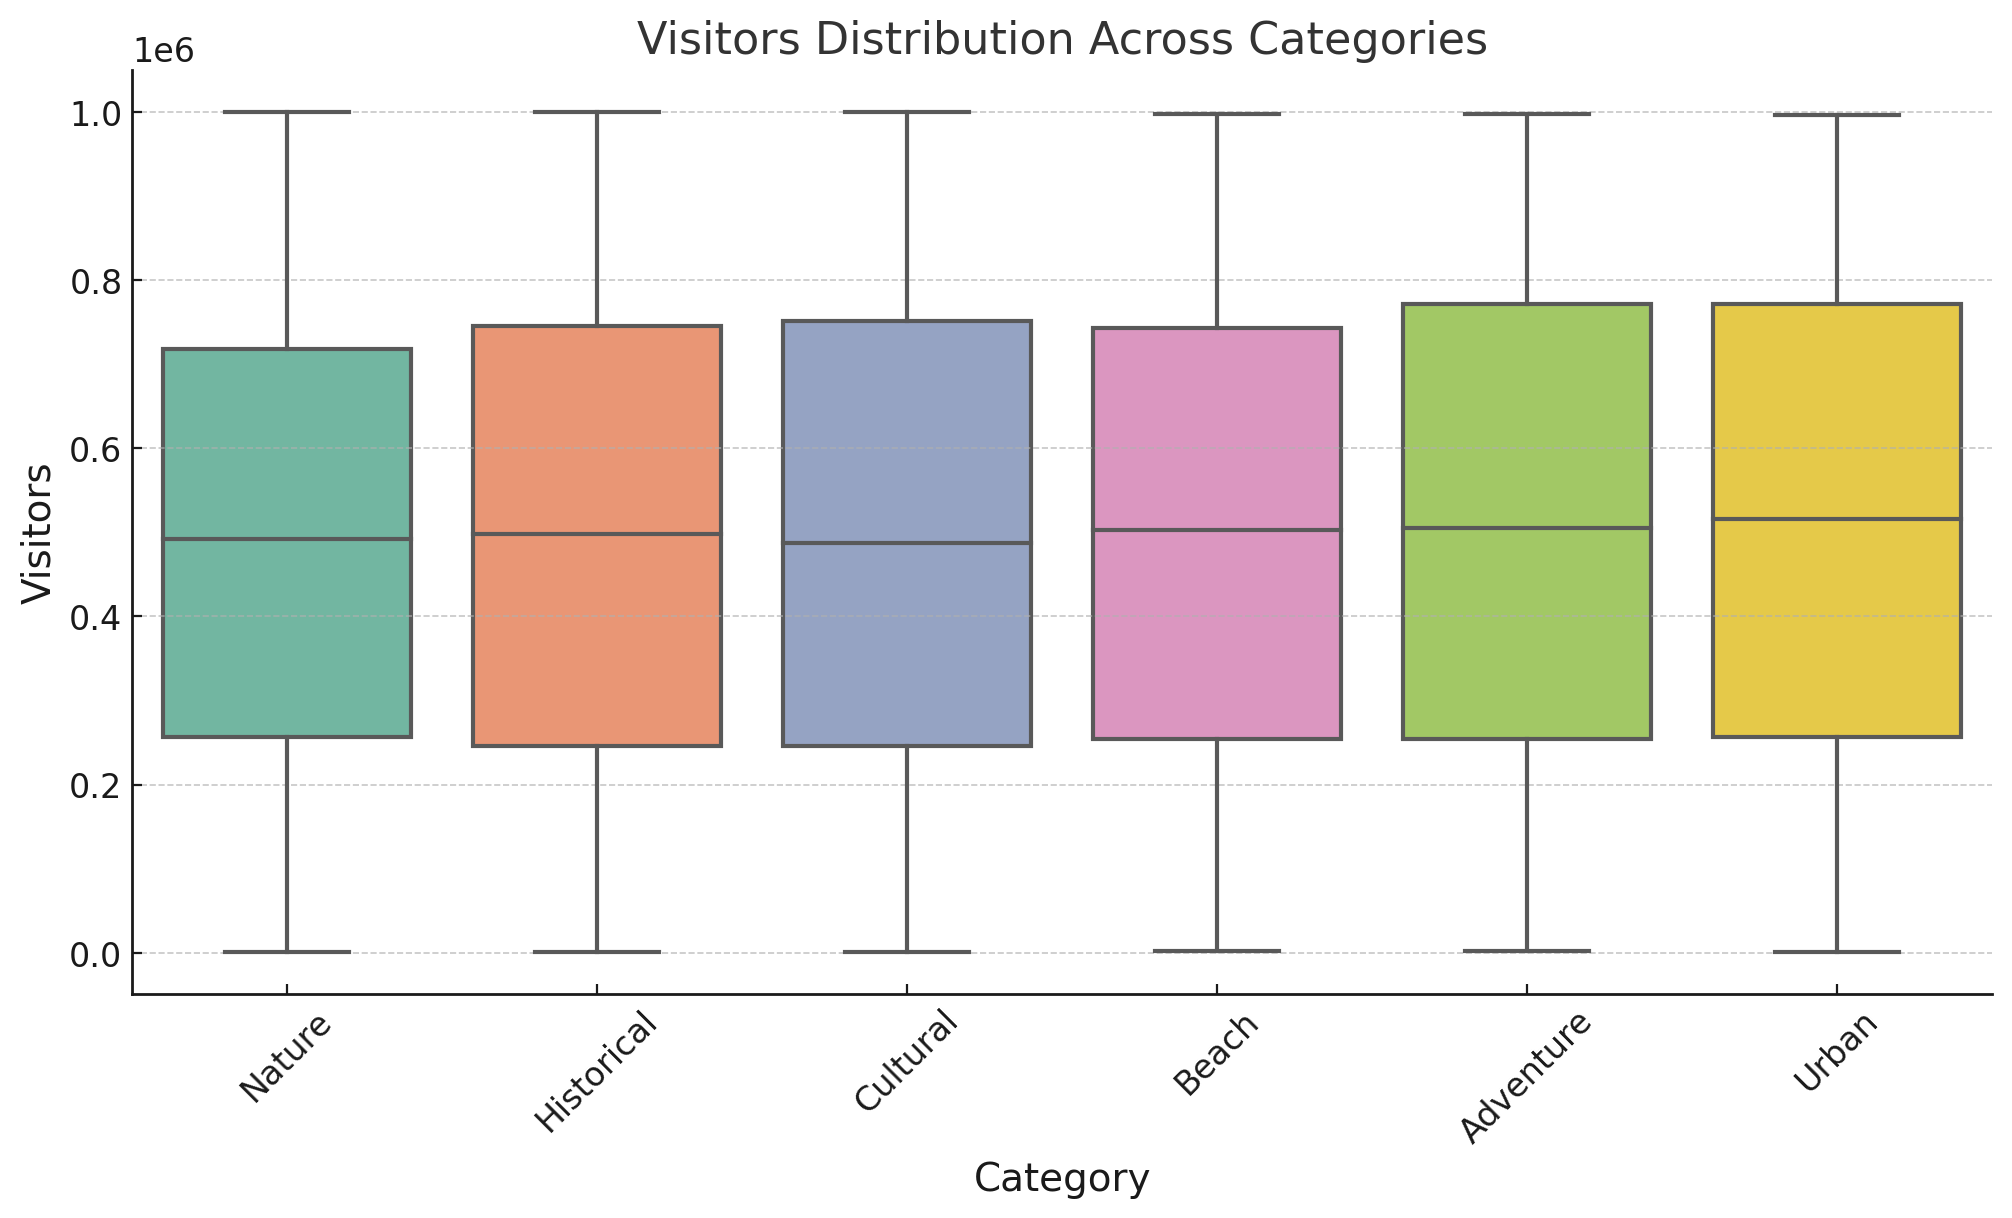
\includegraphics[width=0.8\textwidth]{output (4).png}
    \caption{Visitors Distribution Across Categories}
    \label{fig:visitors_distribution}
\end{figure}

\begin{figure}[h!]
    \centering
    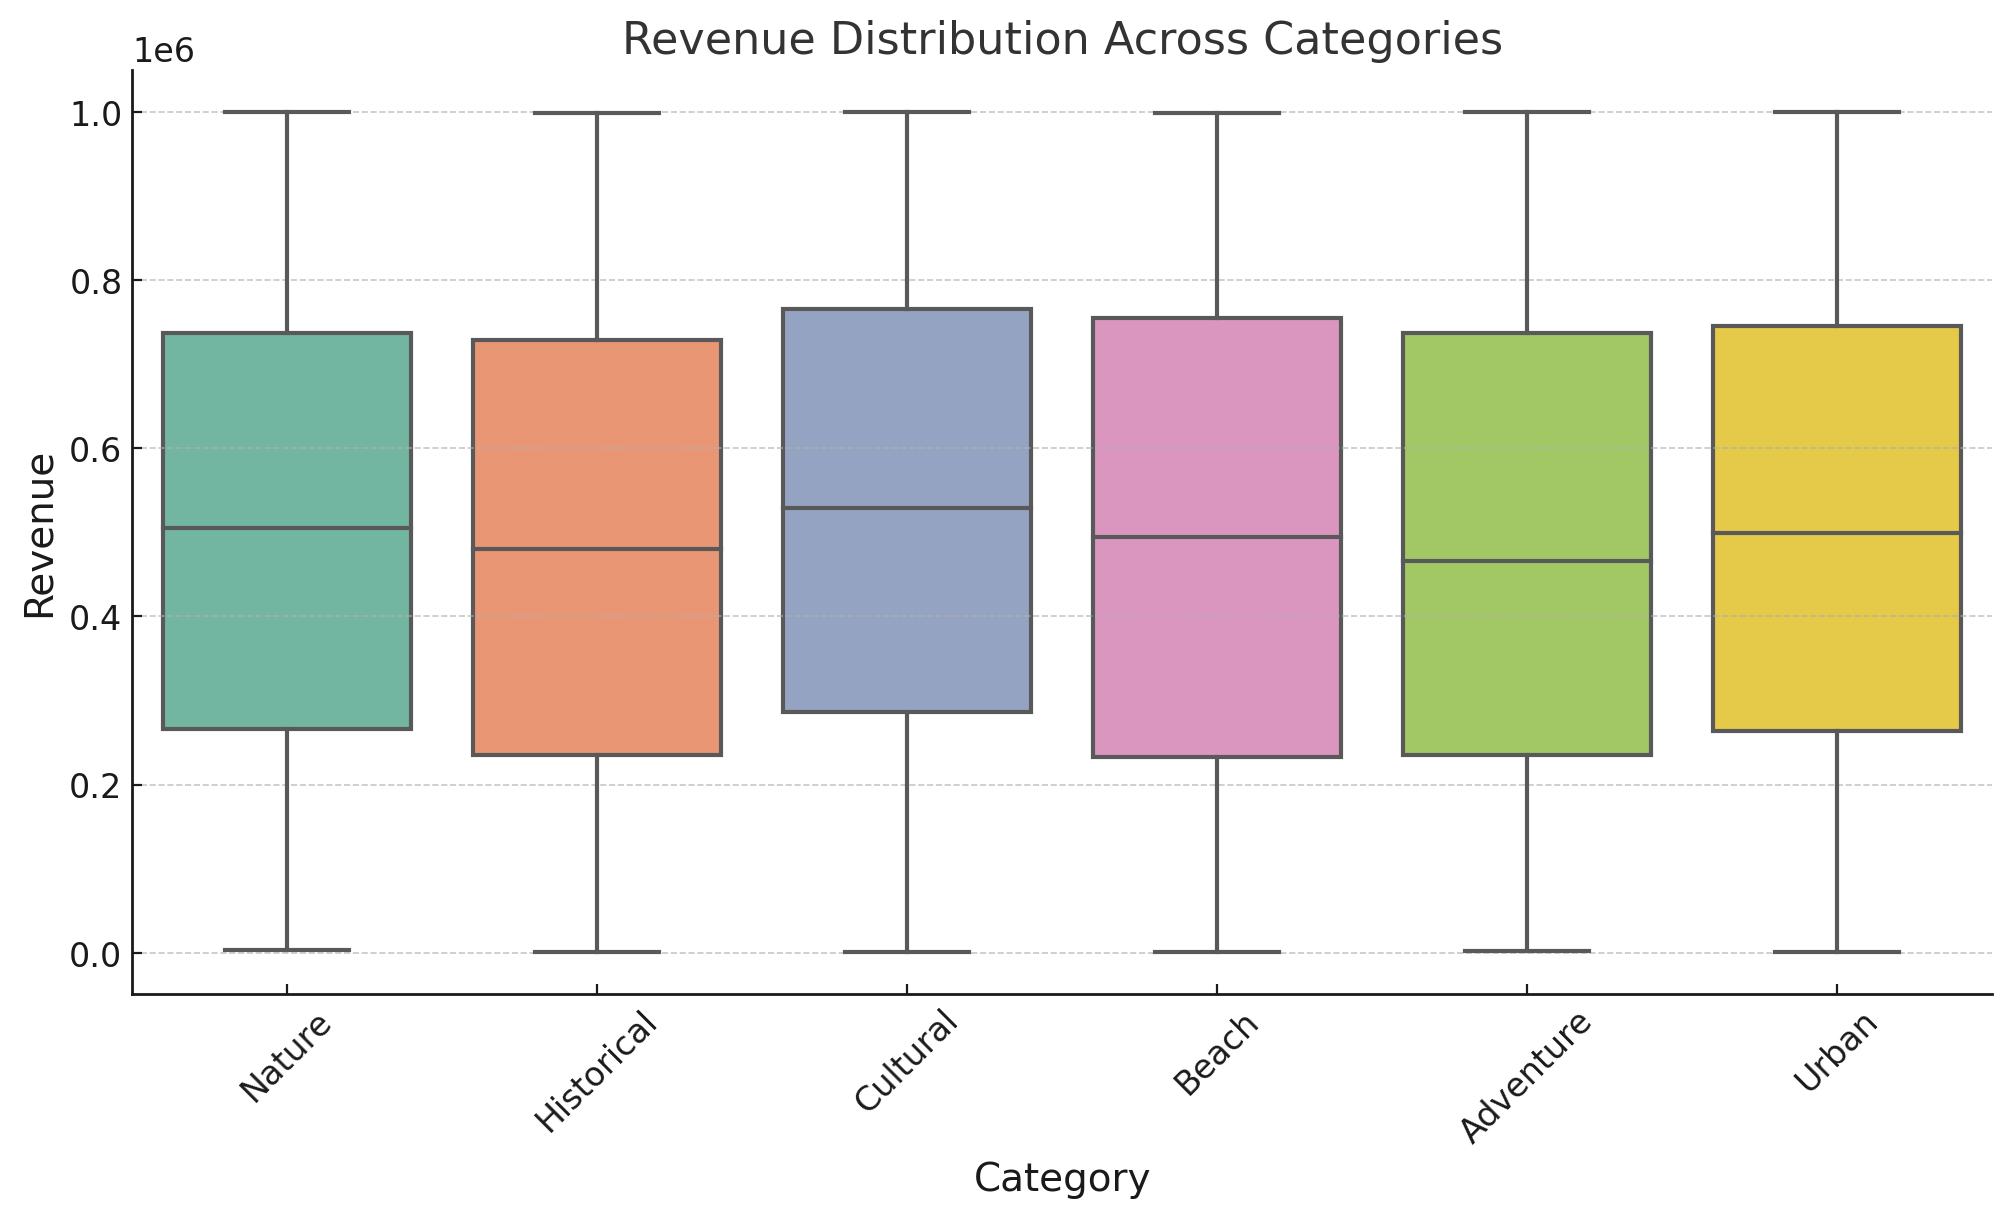
\includegraphics[width=0.8\textwidth]{output (3).png}
    \caption{Revenue Distribution Across Categories}
    \label{fig:revenue_distribution}
\end{figure}

\begin{figure}[h!]
    \centering
    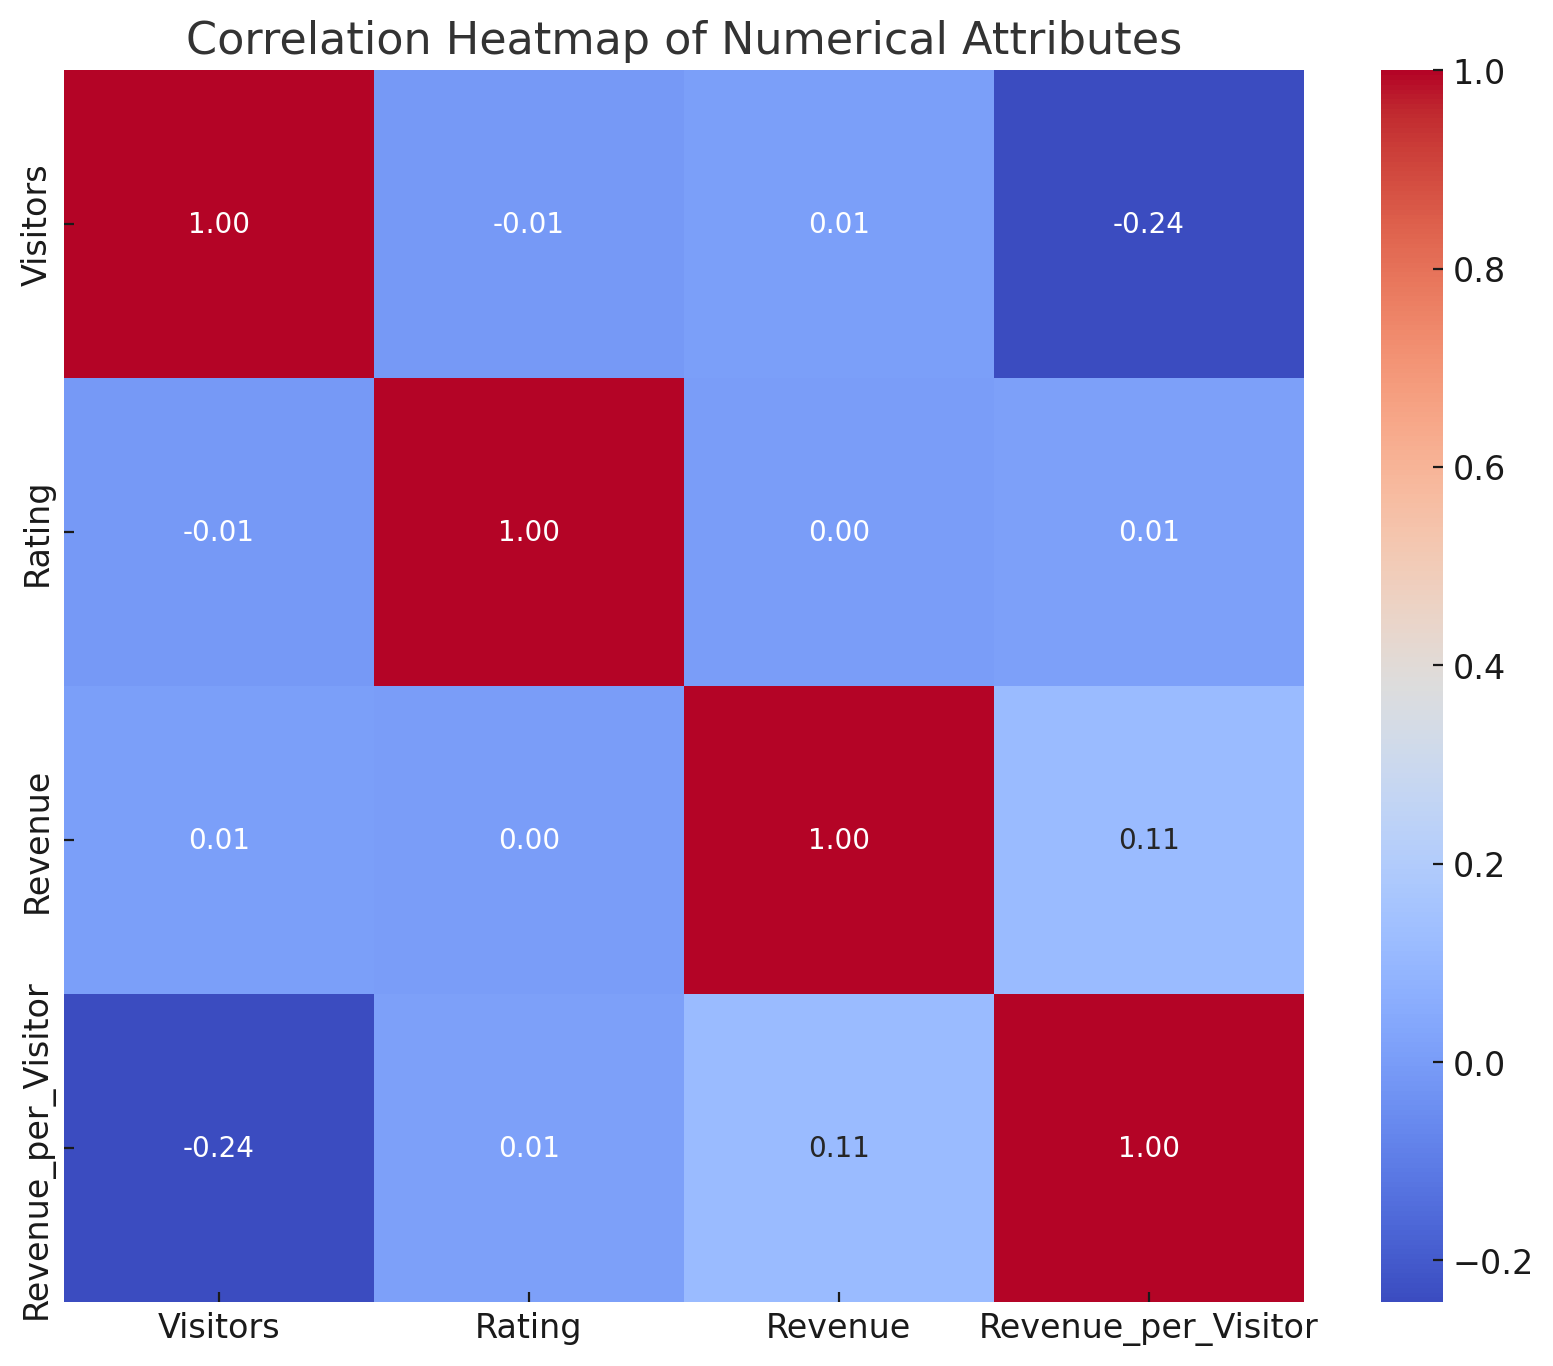
\includegraphics[width=0.6\textwidth]{output (2).png}
    \caption{Correlation Heatmap of Numerical Attributes}
    \label{fig:correlation_heatmap}
\end{figure}


\subsubsection{Conclusion}

The insights derived from the exploratory data analysis provide a foundational understanding of the dataset, which directly aids in addressing the main task of this study. The variability in visitor and revenue distributions across categories highlights the importance of tailoring strategies to individual activity types. For example, focusing on highly popular or high-revenue activities within each category could optimize resource allocation.

The correlation analysis further guides the task by identifying the lack of direct relationships between key attributes. This suggests that more complex, non-linear models may be required to predict outcomes such as revenue or visitor numbers effectively. Additionally, the weak negative correlation between revenue per visitor and total visitors underscores the potential value of niche, high-value activities, which may yield better returns despite lower attendance.

Overall, the results emphasize the need for a nuanced approach to analyzing and optimizing tourism activities, integrating both quantitative trends and qualitative insights.

\end{document}